\chapter{1 Kings 16}

\begin{figure}
  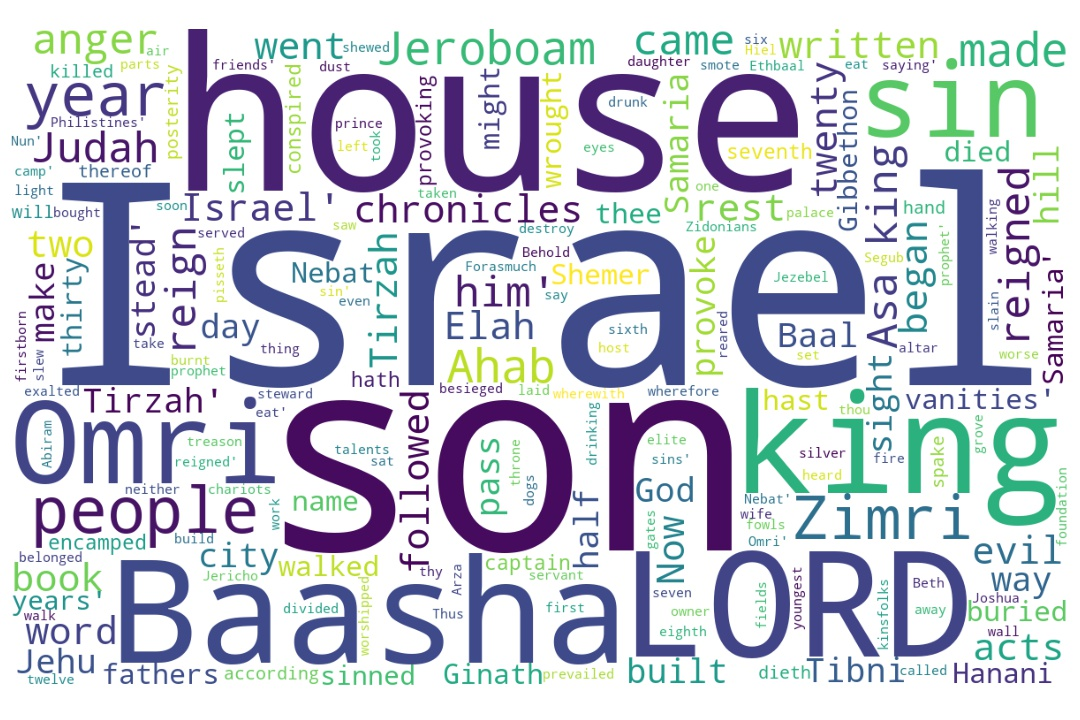
\includegraphics[width=\linewidth]{11OT-1Kings/1Kings16-WordCloud.jpg}
  \caption{1 Kings 16 Word Cloud}
  \label{fig:1 Kings 16 Word Cloud}
\end{figure}

%%%%%%%%%%%%%%%%%%%%%%%%%%%%%%%%%%%%%%%%%
%%%%%%%%%%%%%%%%%%%%%%%%%%%%%%%%%%%%%%%%%

\marginpar{\scriptsize \centering \fcolorbox{bone}{lime}{\textbf{JUST LIKE HEATHEN KINGS}}\\ (1 Kings 16) \begin{compactenum}[I.][8]
     \item The \textbf{Pedigree} \index[scripture]{1Kings!1Ki 16:02} (1Ki 16:2) 
    \item The \textbf{Prince} \index[scripture]{1Kings!1Ki 16:02} (1Ki 16:2) 
    \item The \textbf{Posterity} \index[scripture]{1Kings!1Ki 16:03} (1Ki 16:3) 
    \item The \textbf{Provocations} \index[scripture]{1Kings!1Ki 16:03} \index[scripture]{1Kings!1Ki 16:07}\index[scripture]{1Kings!1Ki 16:77} (1Ki 16:3, 7, 33) 
    \item A \textbf{Pattern} \index[scripture]{1Kings!1Ki 16:07} (1Kis 16:7) 
    \item The \textbf{Purge} \index[scripture]{1Kings!1Ki 16:11} (1Ki 16:11) 
    \item The \textbf{Palace} \index[scripture]{1Kings!1Ki 16:18} (1Ki 16:18) 
    \item The \textbf{Parts} \index[scripture]{1Kings!1Ki 16:21} (1Ki 16:21) 
\end{compactenum}}


\footnote{\textcolor[cmyk]{0.99998,1,0,0}{\hyperlink{TOC}{Return to end of Table of Contents.}}}\footnote{\href{https://audiobible.com/bible/1_kings_16.html}{\textcolor[cmyk]{0.99998,1,0,0}{1 Kings 16 Audio}}}\textcolor[cmyk]{0.99998,1,0,0}{Then the word of the LORD came to Jehu the son of Hanani against Baasha, saying,}
[2] \textcolor[cmyk]{0.99998,1,0,0}{Forasmuch as I exalted thee out of the dust, and made thee prince over my people Israel; and thou hast walked in the way of Jeroboam, and hast made my people Israel to sin, to provoke me to anger with their sins;}
[3] \textcolor[cmyk]{0.99998,1,0,0}{Behold, I will take away the posterity of Baasha, and the posterity of his house; and will make thy house like the house of Jeroboam the son of Nebat.}
[4] \textcolor[cmyk]{0.99998,1,0,0}{Him that dieth of Baasha in the city shall the dogs eat; and him that dieth of his in the fields shall the fowls of the air eat.}
[5] \textcolor[cmyk]{0.99998,1,0,0}{Now the rest of the acts of Baasha, and what he did, and his might, \emph{are} they not written in the book of the chronicles of the kings of Israel?}
[6] \textcolor[cmyk]{0.99998,1,0,0}{So Baasha slept with his fathers, and was buried in Tirzah: and Elah his son reigned in his stead.}
[7] \textcolor[cmyk]{0.99998,1,0,0}{And also by the hand of the prophet Jehu the son of Hanani came the word of the LORD against Baasha, and against his house, even for all the evil that he did in the sight of the LORD, in provoking him to anger with the work of his hands, in being like the house of Jeroboam; and because he killed him.}\\
\\
\P \textcolor[cmyk]{0.99998,1,0,0}{In the twenty and sixth year of Asa king of Judah began Elah the son of Baasha to reign over Israel in Tirzah, two years.}
[9] \textcolor[cmyk]{0.99998,1,0,0}{And his servant Zimri, captain of half \emph{his} chariots, conspired against him, as he was in Tirzah, drinking himself drunk in the house of Arza steward of \emph{his} house in Tirzah.}
[10] \textcolor[cmyk]{0.99998,1,0,0}{And Zimri went in and smote him, and killed him, in the twenty and seventh year of Asa king of Judah, and reigned in his stead.}\\
\\
\P \textcolor[cmyk]{0.99998,1,0,0}{And it came to pass, when he began to reign, as soon as he sat on his throne, \emph{that} he slew all the house of Baasha: he left him not one that pisseth against a wall, neither of his kinsfolks, nor of his friends.}
[12] \textcolor[cmyk]{0.99998,1,0,0}{Thus did Zimri destroy all the house of Baasha, according to the word of the LORD, which he spake against Baasha by Jehu the prophet,}
[13] \textcolor[cmyk]{0.99998,1,0,0}{For all the sins of Baasha, and the sins of Elah his son, by which they sinned, and by which they made Israel to sin, in provoking the LORD God of Israel to anger with their vanities.}
[14] \textcolor[cmyk]{0.99998,1,0,0}{Now the rest of the acts of Elah, and all that he did, \emph{are} they not written in the book of the chronicles of the kings of Israel?}\\\
\\
\P \textcolor[cmyk]{0.99998,1,0,0}{In the twenty and seventh year of Asa king of Judah did Zimri reign seven days in Tirzah. And the people \emph{were} encamped against Gibbethon, which \emph{belonged} to the Philistines.}
[16] \textcolor[cmyk]{0.99998,1,0,0}{And the people \emph{that} \emph{were} encamped heard say, Zimri hath conspired, and hath also slain the king: wherefore all Israel made Omri, the captain of the host, king over Israel that day in the camp.}
[17] \textcolor[cmyk]{0.99998,1,0,0}{And Omri went up from Gibbethon, and all Israel with him, and they besieged Tirzah.}
[18] \textcolor[cmyk]{0.99998,1,0,0}{And it came to pass, when Zimri saw that the city was taken, that he went into the palace of the king's house, and burnt the king's house over him with fire, and died,}
[19] \textcolor[cmyk]{0.99998,1,0,0}{For his sins which he sinned in doing evil in the sight of the LORD, in walking in the way of Jeroboam, and in his sin which he did, to make Israel to sin.}
[20] \textcolor[cmyk]{0.99998,1,0,0}{Now the rest of the acts of Zimri, and his treason that he wrought, \emph{are} they not written in the book of the chronicles of the kings of Israel?}\\
\\
\P \textcolor[cmyk]{0.99998,1,0,0}{Then were the people of Israel divided into two parts: half of the people followed Tibni the son of Ginath, to make him king; and half followed Omri.}
[22] \textcolor[cmyk]{0.99998,1,0,0}{But the people that followed Omri prevailed against the people that followed Tibni the son of Ginath: so Tibni died, and Omri reigned.}\\
\\
\P \textcolor[cmyk]{0.99998,1,0,0}{In the thirty and first year of Asa king of Judah began Omri to reign over Israel, twelve years: six years reigned he in Tirzah.}
[24] \textcolor[cmyk]{0.99998,1,0,0}{And he bought the hill Samaria of Shemer for two talents of silver, and built on the hill, and called the name of the city which he built, after the name of Shemer, owner of the hill, Samaria.}\\
\\
\P \textcolor[cmyk]{0.99998,1,0,0}{But Omri wrought evil in the eyes of the LORD, and did worse than all that \emph{were} before him.}
[26] \textcolor[cmyk]{0.99998,1,0,0}{For he walked in all the way of Jeroboam the son of Nebat, and in his sin wherewith he made Israel to sin, to provoke the LORD God of Israel to anger with their vanities.}
[27] \textcolor[cmyk]{0.99998,1,0,0}{Now the rest of the acts of Omri which he did, and his might that he shewed, \emph{are} they not written in the book of the chronicles of the kings of Israel?}
[28] \textcolor[cmyk]{0.99998,1,0,0}{So Omri slept with his fathers, and was buried in Samaria: and Ahab his son reigned in his stead.}\\
\\
\P \textcolor[cmyk]{0.99998,1,0,0}{And in the thirty and eighth year of Asa king of Judah began Ahab the son of Omri to reign over Israel: and Ahab the son of Omri reigned over Israel in Samaria twenty and two years.}
[30] \textcolor[cmyk]{0.99998,1,0,0}{And Ahab the son of Omri did evil in the sight of the LORD above all that \emph{were} before him.}
[31] \textcolor[cmyk]{0.99998,1,0,0}{And it came to pass, as if it had been a light thing for him to walk in the sins of Jeroboam the son of Nebat, that he took to wife Jezebel the daughter of Ethbaal king of the Zidonians, and went and served Baal, and worshipped him.}
[32] \textcolor[cmyk]{0.99998,1,0,0}{And he reared up an altar for Baal in the house of Baal, which he had built in Samaria.}
[33] \textcolor[cmyk]{0.99998,1,0,0}{And Ahab made a grove; and Ahab did more to provoke the LORD God of Israel to anger than all the kings of Israel that were before him.}\\
\\
\P \textcolor[cmyk]{0.99998,1,0,0}{In his days did Hiel the Beth-elite build Jericho: he laid the foundation thereof in Abiram his firstborn, and set up the gates thereof in his youngest \emph{son} Segub, according to the word of the LORD, which he spake by Joshua the son of Nun.}
